\begin{frame}[t,fragile]{Noise}
    \begin{columns}[t]
        \column{0.6\textwidth}
        \begin{itemize}
            \item Salt and pepper noise: contains random occurrences of black and white pixels
            \item Impulse noise: contains random occurrences of white pixels
            \item Gaussian noise: variations in intensity drawn from a Gaussian normal distribution
        \end{itemize}
        \column{0.4\textwidth}
            \begin{figure}
              \centering
              %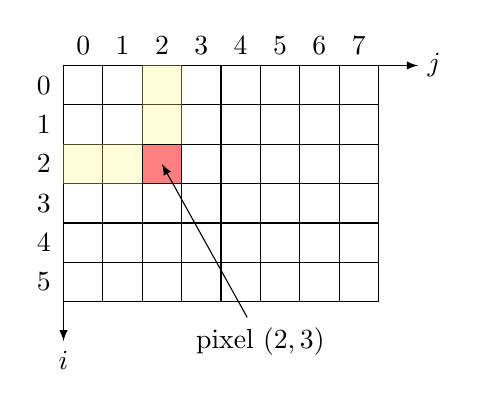
\begin{tikzpicture}[scale=0.5]
	\foreach \i in {0,1,...,6}
	{
		\draw (0,\i) -- ++(8,0);
	}
	\foreach \i in {0,1,...,5}
	{
		\node at (-0.5, 5.5 - \i) {$\i$};
	}	
	\foreach \j in {0,1,...,8}
	{
		\draw (\j,0) -- ++(0,6);
	}
	\foreach \j in {0,1,...,7}
	{
		\node at (\j + 0.5, 6.5) {$\j$};
	}		
	\draw[-latex] (0,6) -- ++(0,-7) node[anchor=north] {$i$};		
	\draw[-latex] (0,6) -- ++(9,0) node[anchor=west] {$j$};

    \pause
    \draw [draw=none, fill=yellow!50, opacity=0.3] (0,3) rectangle (3,4);
    \draw [draw=none, fill=yellow!50, opacity=0.3] (2,3) rectangle (3,6);
    \draw[fill=red!50] (2,3) rectangle ++(1,1);
    \node (a) at  (5,-1) {pixel $(2,3)$};
    \draw[-latex] (a) -- (2.5,3.5);
	
\end{tikzpicture} 
              \caption{}
            \end{figure}
    \end{columns}
        \credit{S. Sietz}
\end{frame}


\begin{frame}[t,fragile]{Gaussian Noise}
    \begin{columns}[t]
        \column{0.5\textwidth}
        \begin{itemize}
            \item Mathematical model: sum of many independent factors
            \item Good for small standard deviations
            \item Assumption: independent, zero-mean noise
        \end{itemize}
        \column{0.5\textwidth}
            \begin{figure}
              \centering
              \includegraphics[width=\textwidth]{./figures/gaussian_noise.jpg}
              \caption{}
            \end{figure}
    \end{columns}
        \credit{M. Hebert}
\end{frame}


\begin{frame}[plain]
    \begin{columns}[t]
        \column{0.5\textwidth}
        \begin{figure}
          \centering
          \includegraphics[width=\textwidth]{./figures/noise_level_and_smoothing.jpg}
          \caption{Reducing Gaussian noise: noise $\sigma$ and smoothing kernel size}
        \end{figure}
        \column{0.5\textwidth}
            \vspace{0.5in}
            Reducing Gaussian Noise\par
            Smoothing with larger standard deviations suppresses noise, but also blurs the image.
    \end{columns}
        \credit{Svetlana Lazebnik}
\end{frame}



\begin{frame}{Reducing Salt-and-Pepper Noise}
    \begin{figure}
      \centering
      \includegraphics[width=\textwidth]{./figures/s_and_p_with_gaussian.jpg}
      \caption{Inability to reduce salt and pepper noise with Gaussian filtering}
    \end{figure}
\end{frame}


\begin{frame}{Median Filtering}

    \begin{columns}[t]
        \column{0.6\textwidth}
        \begin{figure}
          \centering
          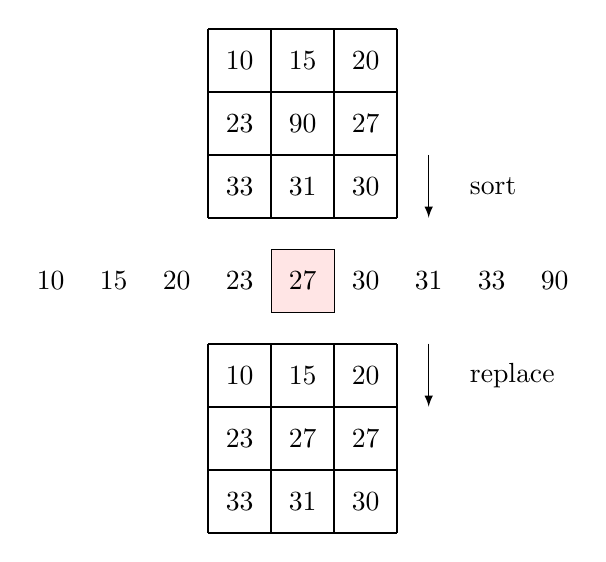
\begin{tikzpicture}[scale=0.8]

\draw [thick, step=1cm] (0,0) grid (3,3);
\foreach \i/\v in {0/33, 1/31, 2/30, 3/23, 4/90, 5/27,6/10, 7/15, 8/20}
{	
	\pgfmathparse{round(mod(\i,3)) + 0.5};
	\let\x\pgfmathresult;
	\pgfmathparse{round(div(\i,3)) + 0.5};
	\let\y\pgfmathresult;	
	\node at (\x, \y) {\v};
}
\draw[-latex] (3.5, 1) -- ++(0,-1);
\node [anchor=west] at (4, 0.5) {sort};

\draw[fill=red!10] (1, -1.5) rectangle ++(1,1);
\foreach \i/\v in {0/10, 1/15, 2/20, 3/23, 4/27, 5/30, 6/31, 7/33, 8/90}
{
	\node at (-2.5 + \i, -1) {\v};
}



\draw[-latex] (3.5, -2) -- ++(0,-1);
\node [anchor=west] at (4, -2.5) {replace};


\draw [thick, step=1cm] (0,-5) grid++ (3,3);
\foreach \i/\v in {0/33, 1/31, 2/30, 3/23, 4/27, 5/27,6/10, 7/15, 8/20}
{	
	\pgfmathparse{round(mod(\i,3)) + 0.5};
	\let\x\pgfmathresult;
	\pgfmathparse{round(div(\i,3)) + 0.5 -5};
	\let\y\pgfmathresult;	
	\node at (\x, \y) {\v};
}
\end{tikzpicture}
          \caption{}
        \end{figure}
        \column{0.4\textwidth}
        A median filter operates over a window by selecting the median intensity in the window. \\
        Is median filtering linear?
        \credit{K. Grauman} 
    \end{columns}
    
\end{frame}

\begin{frame}{Sharpening Revisited}

    \begin{columns}[t]
        \column{0.6\textwidth}
        \begin{figure}
          \centering
          \includegraphics[width=\textwidth]{./figures/tom_unsharp.jpg}
          \caption{Sharpening}
        \end{figure}
        \column{0.4\textwidth}
        \begin{enumerate}
            \item What does blurring take away?
            \item We add it back.
        \end{enumerate}
        \credit{Svetlana Lazebnik}
    \end{columns}
\end{frame}

\begin{frame}{Unsharp Mask Filter}
    \begin{equation*}
        f + \alpha(f - f\ast g) = (1+\alpha)f - \alpha f\ast g = f\ast ((1+\alpha)e - g)
    \end{equation*}
    
\end{frame}